\section{Arreglo de compuertas OR, AND y XOR en Verilog \label{sec:s3}}

\begin{center}
	\begin{minipage}{12cm}
		\begin{tcolorbox}[title=Actividad 3]
			Obtener la versión “verilog” de los 2 códigos VHDL mostrados en esta tarea. Observar el resultado con el visor RTL.
		\end{tcolorbox}	
	\end{minipage}
\end{center}

La visualización RTL del arreglo de compuertas OR (primer código), descrito en Verilog, se muestra en la \autoref{fig:forgenerate1_verilog_rtl}. La implementación se hace instanciando 8 veces al módulo denominado ``MyOr2'' (debido a que las dos entradas son de 8 bits), que simplemente es una compuerta OR de 1 bit (ver \autoref{fig:forgenerate1_verilog_rtl2}). Las simulaciones se visualizan en la \autoref{fig:forgenerate1_verilog_wave}, en donde se muestra que este arreglo de compuerta OR opera de manera correcta.

En los Anexos se localiza la descripción en VHDL del primer código. Primeramente se crea el módulo que se va a instanciar (compuerta OR), declarando las entradas y salidas, así como la descripción de su comportamiento. Después se declara al módulo principal, con las entradas y salidas de este. Se debe declarar a la variable de iteración ``n'', para después utilizar a la estructura \textit{for-generate} e instanciar 8 veces al primer módulo descrito (debido a que las entradas son de 8 bits)

La visualización RTL del arreglo de compuertas OR, AND y XOR (segundo código), descrito en Verilog, se muestra en la \autoref{fig:forgenerate2_verilog_rtl}. La implementación se hace nuevamente instanciando 8 veces al módulo denominado ``MyOr2'', no obstante, se agregan 4 instancias de compuertas AND para los 4 bits menos significativos de las entradas A y B, y otras 4 instancias de compuertas XOR para los 4 bits más significativos (ver \autoref{fig:forgenerate2_verilog_rtl2}). Las simulaciones se visualizan en la \autoref{fig:forgenerate2_verilog_wave}, en donde se muestra que este arreglo de compuertas OR, AND y XOR opera de manera correcta.

En los Anexos se localiza la descripción en VHDL del segundo código. Se realiza lo mismo que en el primer código, no obstante, se deben declarar 3 variables de iteración (una por cada ciclo) y solo es necesario emplear una estructura \textit{for-generate} y dos estructuras \textit{for} para separar a los 4 bits más y menos significativos e instanciar las compuertas AND y XOR. 

\begin{figure}[ht]
	\centering
	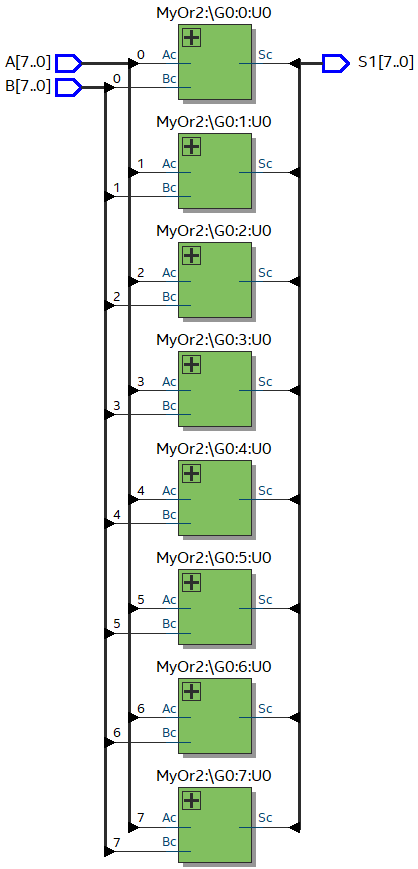
\includegraphics[scale=0.95]{ForGenerate1_VHDL_RTL.png}
	\caption{Diagrama RTL del arreglo de compuertas OR, descrito en VHDL. \label{fig:forgenerate1_verilog_rtl}}
\end{figure}

\begin{figure}[ht]
	\centering
	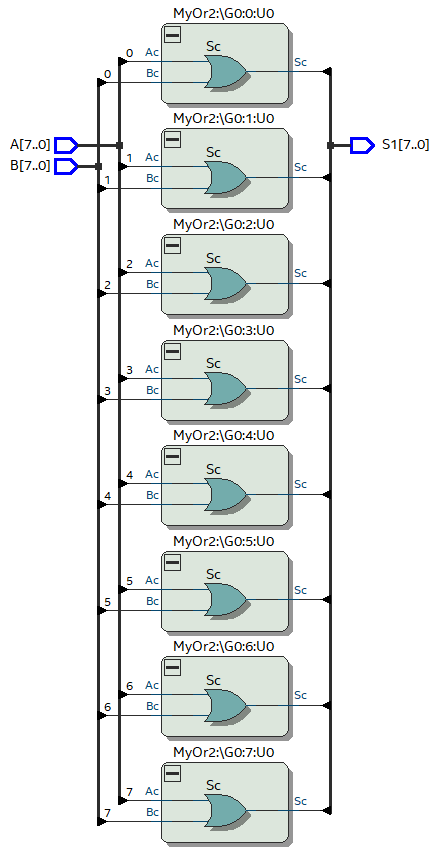
\includegraphics[scale=0.95]{ForGenerate1_VHDL_RTL2.png}
	\caption{Diagrama RTL del arreglo de compuertas OR, descrito en VHDL (vista interna de las instancias). \label{fig:forgenerate1_verilog_rtl2}}
\end{figure}

\begin{figure}[ht]
	\centering
	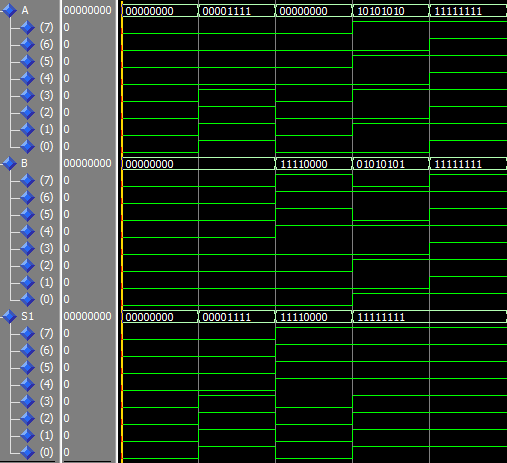
\includegraphics[scale=1.25]{ForGenerate1_VHDL_Wave.png}
	\caption{Simulación del arreglo de compuertas OR, descrito en VHDL, con el visor de formas de onda de ModelSim. \label{fig:forgenerate1_verilog_wave}}
\end{figure}

\begin{figure}[ht]
	\centering
	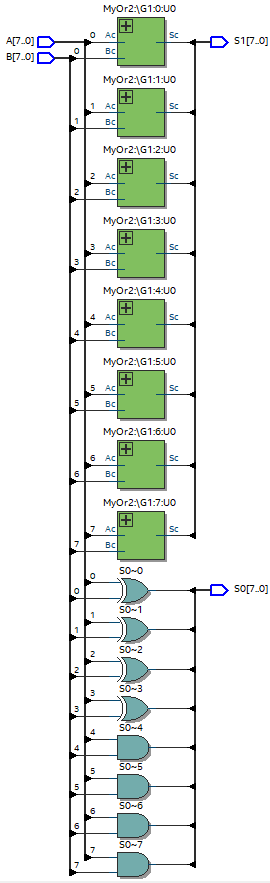
\includegraphics[scale=0.95]{ForGenerate2_VHDL_RTL.png}
	\caption{Diagrama RTL del arreglo de compuertas OR, AND y XOR, descrito en VHDL. \label{fig:forgenerate2_verilog_rtl}}
\end{figure}

\begin{figure}[ht]
	\centering
	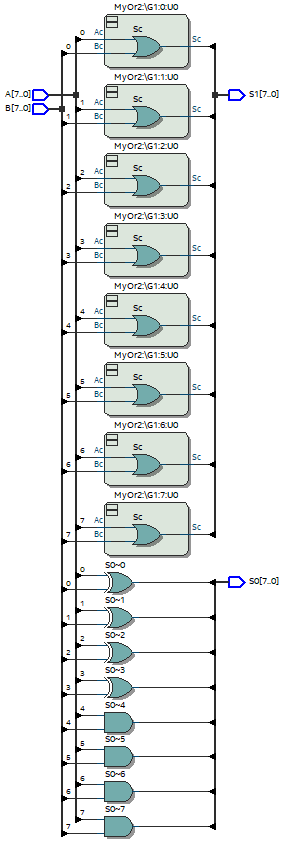
\includegraphics[scale=0.95]{ForGenerate2_VHDL_RTL2.png}
	\caption{Diagrama RTL del arreglo de compuertas OR, AND y XOR, descrito en VHDL (vista interna de las instancias). \label{fig:forgenerate2_verilog_rtl2}}
\end{figure}

\begin{figure}[ht]
	\centering
	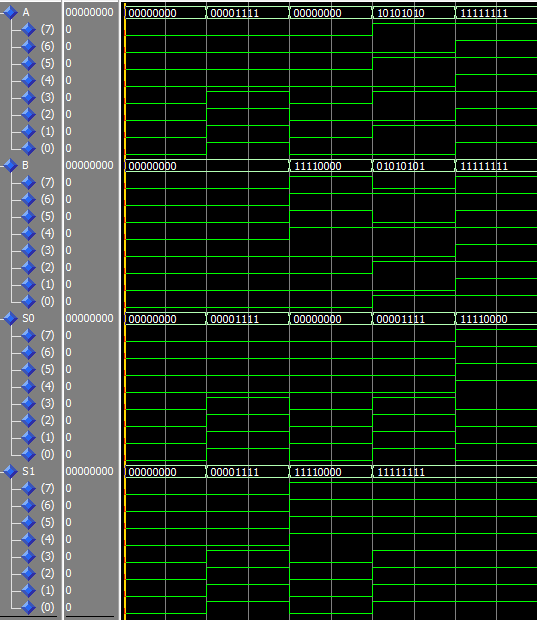
\includegraphics[scale=1.15]{ForGenerate2_VHDL_Wave.png}
	\caption{Simulación del arreglo de compuertas OR, AND y XOR, descrito en VHDL, con el visor de formas de onda de ModelSim. \label{fig:forgenerate2_verilog_wave}}
\end{figure}